%Cloud-Computing Basics a Non tech. intro.
%Seite 163
% Wie werden die Informationen die Benutzer gezeigt und wie können sie diese manipulieren
%[Rev]
In diesem Kapitel werden die Optimierungsmaßnahmen für EC2-Instanzen und Amazon S3 vorgestellt. Es wird gezeigt, wie man mithilfe von CloudWatch und Cost-Explorer, die Effekte der Optimierungsmaßnahmen messen kann. Somit kann ein Vergleich zwischen den Kosten vor und nach der Optimierungsmaßnahmen durchgeführt werden.
%Die mit den Überwachungswerkzeuge gesammelte Informationen, bilden die Grundlage für die Optimierungsmaßnahmen für EC2-Instanzen und Amazon S3.
%Wenn zum Beispiel festgestellt wird, dass Instanzen nicht ausreichend genutzt werden, können sie so konfiguriert werden, dass sie abgeschaltet werden.
%La mayoria de las medidas de opmimizacion se centran en las instancias EC2, pues como antes mencionado representan la gran mayoria de los servicios que comprenden los gastos en nuestras facturas.

\subsection{EC2 Auto Scaling}
%t.ly/CXs3 Linked In auf DE          %t.ly/1nka          %THIS!!! t.ly/vrCO
%https://youtu.be/qYHR_V1lvNU?t=900
Das \textit{Auto Scaling} oder die automatische Skalierung von Instanzen dient dazu die richtige Anzahl von EC2-Instanzen zur Verfügung zu haben, um die Anwendungslast dynamisch abzudecken.\footnote{Vgl. AWS, 2021, Was ist Amazon EC2 Auto Scaling? S.9\cite{AMZ31}} Diese Fähigkeit wird als \textit{horizontale Skalierung} bezeichnet.\footnote{Die Grundbedeutung der horizontalen Skalierung ist, dass Systeme durch zusätzliche Komponenten erweitert werden. Im Gegensatz dazu bedeutet der Begriff "vertikale Skalierung", dass einer einzelnen Komponente zusätzliche Leistungsfähigkeiten und Ressourcen hinzugefügt werden.(Vgl. Techopedia, 2021, Definition von Horizontal Scaling
, o.S.\cite{TECH1}) }
\\\\
Die \autoref{fig:AutoSca_Unused_Capacity} zeigt das wechselnde Verhalten einer Beispielanwendung, die vor allem unter der Woche genutzt wird. Am Wochenende sinkt die Nachfrage nach Rechnerkapazität auf weniger als 25\% und lässt den Rest der Kapazitäten ungenutzt. 
\begin{figure}[h]
    \centering
    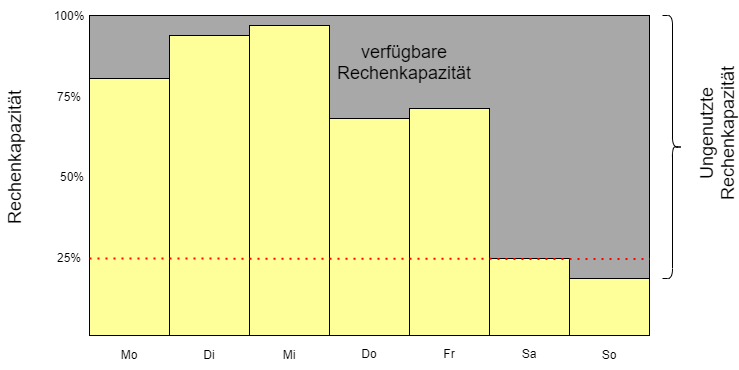
\includegraphics[scale=0.5]{sources/AutoCap Unused Capacity}
    \caption[Ungenutzte Rechenkapazität ohne automatische Skalierung]{}
    \label{fig:AutoSca_Unused_Capacity} Ungenutzte Rechenkapazität ohne automatische Skalierung. \\
    Quelle: Eigene Darstellung mit fiktiven Angaben. 
    %\footnote{\cite{AMZ01}}
  \end{figure}\\
Die gelben Säulen stellen die tägliche genutzte Rechenkapazität dar.
Die graue Zone entspricht ungenutzte Rechenkapazität und beträgt etwa ein Drittel der wöchentlichen Rechnerkapazität.
\subsubsection*{Auto Scaling Group}
Die Instanzen, die zur Deckung der erforderlichen Rechenkapazität zur Verfügung stehen, werden in einer \textit{Auto-Scaling-Gruppe (Auto Scaling Group)} zusammengefasst. Diese Gruppe von Instanzen wird in AWS als Auto-Scaling-Gruppe bezeichnet. Bei der Erstellung einer Auto-Scaling-Gruppe wird somit eine minimale, gewünschte und maximale Anzahl von Instanzen definiert. 
\\\\
Die \autoref{fig:BA Diagramme-AutoScaling and LoadBalancer.drawio} zeigt die gewünschte Instanzen einer Auto-Scaling-Gruppe, welche beim Start der Auto-Scaling-Gruppe gestartet werden. Die minimale und maximale Anzahl von Instanzen sind die Grenzwerte für die Auto-Scaling-Gruppe.  
\begin{figure}[h]
  \centering
  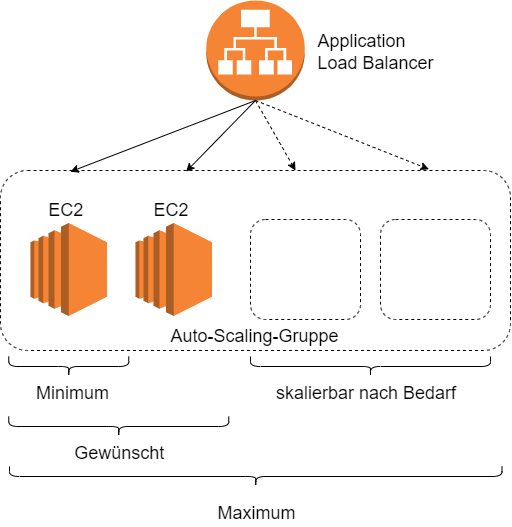
\includegraphics[scale=0.5]{sources/BA Diagramme-AutoScaling and LoadBalancer.drawio}
  \caption[Auto-Scaling-Gruppe nach den Anzahl der Instanzen und Umleitung der Datenverkehr durch dem Application Load Balancer]{}
  \label{fig:BA Diagramme-AutoScaling and LoadBalancer.drawio} 
  Auto-Scaling-Gruppe nach den Anzahl der Instanzen und\\ die Umleitung der Datenverkehr durch dem Application Load Balancer.\\
  Quelle: Eigene Darstellung %mit fiktiven Angaben. 
  basiert auf Amazon \\
  EC2 Auto Scaling - Benutzerhandbuch. S.9\cite{AMZ31}.
\end{figure}
%https://www.youtube.com/watch?v=yC5nRYS2IYI En Espaniol
%https://docs.aws.amazon.com/autoscaling/ec2/userguide/as-scaling-simple-step.html#policy-creating-asg-console
\\\\
%Zu erklären: cooldown period and scaling policy.
%Macht die Nutzung von Spor-Instanzen so einfach wie nie zuvor ?
\subsubsection*{Elastic Load Balancing}
%[Rev]
%https://docs.aws.amazon.com/autoscaling/ec2/userguide/autoscaling-load-balancer.html
%Durch einem \textit{Elastic Load Balancer} wird den eingehenden Anwendungsverkehr automatisch auf alle laufenden EC2-Instanzen verteilt. 
Ein \textit{Elastic Load Balancer} ist für die Verwaltung eingehender Anfragen zuständig, indem es den Datenverkehr auf alle laufenden EC2-Instanzen umleitet.\footnote{In diesem Fall beschränkt auf den Application Load Balancer. (Vgl. AWS, 2021, Amazon Elastic Container Service Entwicklerhandbuch - Load Balancer-Typen -, S.617\cite{AMZ39})} Dies sorgt dafür, dass die Instanzen mit einem ausgeglichener CPU-Auslastung arbeiten. Im diesem Sinne zeigt die \autoref{fig:BA Diagramme-AutoScaling and LoadBalancer.drawio} einen Application-Load-Balancer, welcher den Datenverkehr auf die Instanzen einer Auto-Scaling-Gruppe verteilt.

\subsubsection{Zeitgesteuerte Skalierung}\label{ssec:ZeitgesteuerteScal}
%W-Ende für Dev und Beta
%\textbf{Nicht produktive Umgebungen}\\
%Auch möglich damit https://aws.amazon.com/de/solutions/implementations/instance-scheduler/
In einem On-Premise-System würde es, wenn überhaupt, nur einen geringen Kostenunterschied ausmachen, wenn Instanzen die ganze Zeit aktiv bleiben.\footnote{Anders Lisdorf, 2021, S. 153\cite{CCB}} %\footnote{Vgl. ,Cloud Computing Basics: a Non.-Technical Introduction. Seite 153}. 
Im Gegensatz dazu, ist es bei On-Demand-Zahlungsmodelle sinnvoll Zeiträume zu definieren, in denen Instanzen abgeschaltet werden können, um deren Nutzung zu reduzieren. Bei Systemen, die nur tagsüber und unter der Woche in Betrieb sein müssen, kann sogar dies zu einer Einsparung von bis zu 67\% der Kosten für Instanzen führen. Im Falle, das zum Beispiel Test- und Beta-Umgebungen von Montag bis Freitag von 7 bis 20 Uhr laufen würden. 
\\\\
Die \autoref{fig:Einsparung_Zeitgesteuerte_Skalierung} zeigt die Kostenberechnung einer nicht produktiven Umgebung (z.B. Test, Dev oder Beta) mit On-Demand-Instanzen. Diese Umgebung wird nur von Montag bis Freitag von 7:00 bis 20:00 Uhr genutzt. In der rechten Spalte werden die Kosten für Instanzen berechnet, wenn sie immer aktiv bleiben. In der linken Spalte wurde eine Berechnung durchgeführt, bei der die Instanzen nur dann eingeschaltet werden, wenn sie nach einem Zeitplan gesteuert würden. Darüber hinaus veranschaulicht die \autoref{fig:Einsparung_Zeitgesteuerte_Skalierung} am Ende den Prozentsatz und den Betrag (in Euros) der möglichen Einsparungen, wenn die Instanzen nach einem determinierten Zeitplan gesteuert wird.
\begin{figure}[h]
  \centering
  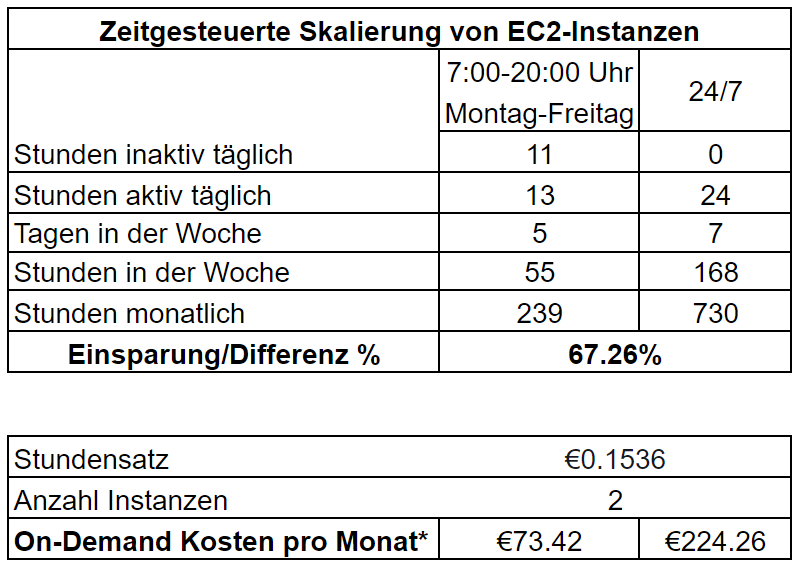
\includegraphics[scale=0.8]{sources/Einsparung_Zeitgesteuerte_Skalierung}
  \caption[Berechnung für ein nicht produktives Umgebung mit zeitgesteuerter Skalierung]{}
  \label{fig:Einsparung_Zeitgesteuerte_Skalierung} 
  Berechnung für ein nicht-produktive Umgebung mit zeitgesteuerter Skalierung. \\
  Quelle: Eigene Darstellung.
\end{figure}
\\\\
\\\\
\\\\
\\\\ 
Quelle des Stundensatzes: AWS Pricing Calculator.\footnote{Der Stundensatz wurde am 23.11.2021 mit dem AWS Pricing Calculator ermitellt für Linux Instanzen in Frankfurt mit 4vCPUs, 16 GB Arbeitsspeicher und Instanz-Familie t4g.xlarge in On-Demand-Zahlungsmodell\cite{AMZ17}.}
% Automatisiere das Hoch- und Herunterfahren von Instanzen
% https://www.linkedin.com/learning/monitoring-aws-with-cloudwatch/autoscaling-using-alarms?autoAdvance=true&autoSkip=true&autoplay=true&resume=false&u=79182202
% Grund: weil i.d.R., kein Entwickler 24/7 arbeitet.
% Wie?: mit Tagging, Lambda oder mit Auto Scaling Groups.
%Wann ist es sinnvoll Systeme runterzufahren 
%HIER LESEN {\cite{CCB}, Seite 153}
%Weihnachten und BackFriday
%\textbf{Produktive Umgebungen}\\
%Wenn der Zeitpunkt einer hohen Nachfrage bekannt ist, kann eine Erhöhung der Rechnerkapazität geplant werden, um Überlastungen zu vermeiden. Beispiele für solche Zeiträume sind Cyber-Monday und Black Friday\footnote{Vgl. Wie viel planen Sie am Black Friday / Cyber Monday auszugeben?\cite{STA5}}. 
%https://de.statista.com/statistik/daten/studie/1076963/umfrage/ausgaben-an-black-friday-und-cyber-monday-in-deutschland/]
\newpage
\subsubsection{Dynamisches Auto Scaling}
%[Rev]
%Intro mit Beispiel
Es kann jedoch zu schnellen und kontinuierlichen Änderungen im Verhalten von Applikationen kommen, häufig innerhalb von wenige Minuten. Bei solchen Szenarien ist es daher sinnvoller, Metriken zur automatischen Anpassung der Skalierung der Rechenkapazität festzulegen. Beispiele für eine veränderte Nutzung von Applikationen finden sich bei \textit{Tinder} und \textit{OkCupid}, zwei der größten Dating-Applikationen in den Vereinigten Staaten. 
\\\\
Die \autoref{fig:Use_by_hour_netflix_OkCupid_tinder} zeigt die Nutzungsspitzen bei den genannten Applikationen. Dieses wechselnde Verhalten wirkt sich unmittelbar auf die zu verschiedenen Tageszeiten benötigte Rechenkapazität aus und macht eine dynamische Skalierung der Rechenkapazität passend, wenn das Ziel darin besteht, ungenutzte Cloud-Dienste abzuschalten. Als Konsequenz der Abschaltung von ungenutzten Cloud-Diensten folgt die Reduzierung von Kosten.
\begin{figure}[h!]
  \centering
  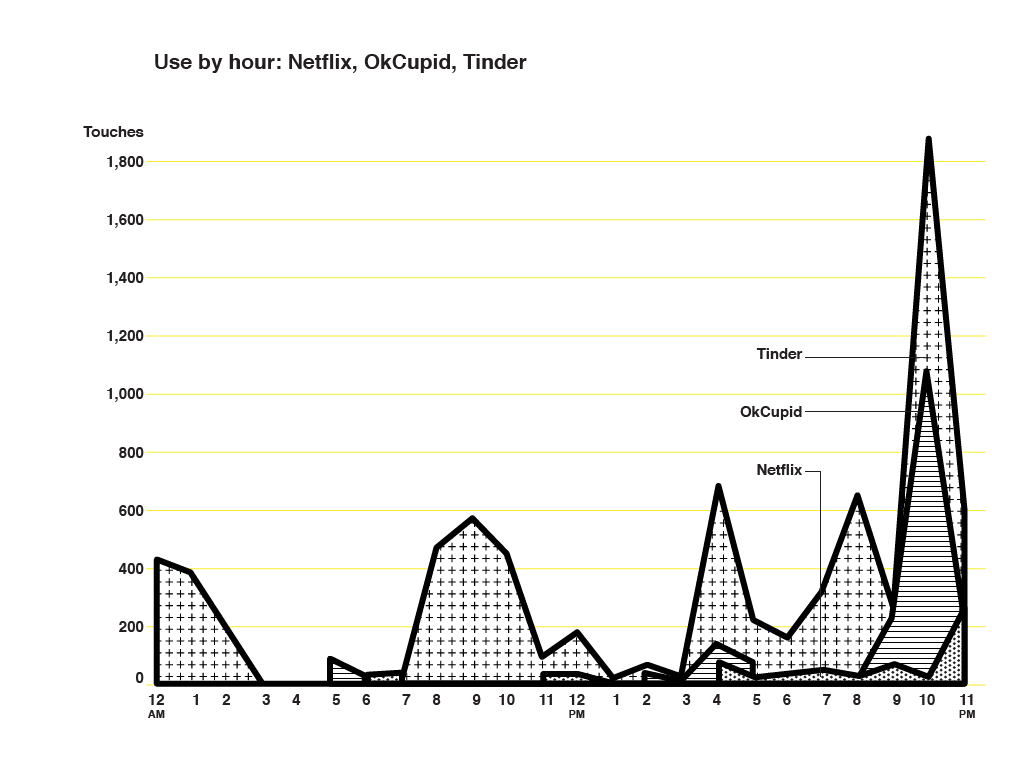
\includegraphics[scale=0.4]{sources/Use_by_hour_netflix_OkCupid_tinder}
  \caption[Nutzung von Tinder, OkCupid und Netflix pro Stunde]{}\label{fig:Use_by_hour_netflix_OkCupid_tinder} 
  DScout's Study: "Putting a Finger on Our Phone Obsession". \\
  Nutzung pro Stunde von Netflix, OkCupid und Tinder während des Tages\cite{SCOUT1}.
  %Quelle: Eigene Darstellung. 
  \\Mit Touches sind die Anzahl der Klicks, Swipes oder einfachen Interaktionen mit der Applikation gemeint.
\end{figure}
\\
Eine der Metriken, die von AWS %[TELEFONAT mit Deepak von der Einheit CIS[Cloud Capgemini]]
benutzt wird, ist die gesamte CPU-Auslastung (CPU-Utilization).\footnote{Die für die automatische Skalierung erforderlichen Metriken wurden bereits ausführlicher im Unterkapitel~\ref{ssec:CloudWatch} erläutert.}
Um die CPU-Auslastung als Metrik zu verwenden, werden mindestens zwei Schwellenwerte definiert, eine für die Erhöhung von Rechenkapazität, \textit{Scale-Out} genannt und eine für das Verringern von Rechenkapazität bezeichnet als \textit{Scale-In}.

\subsubsection{Manual Scaling}
%CHECK/23.11\\
Für die Konfiguration einer Auto-Scaling-Gruppe werden die minimale, maximale und gewünschte Anzahl von Instanzen definiert. Wenn aufgrund von Bedingungen, die in der Konfiguration einer Auto-Scaling-Gruppe nicht berücksichtigt wurden, eine Anpassung in der Rechenkapazität benötigt wird, besteht die Möglichkeit die Rechenkapazität manuell zu steuern. Dies geschieht, ohne dass die aktiven Instanzen unterbrochen werden.

\subsubsection{Predective Scaling}%Voraussagende Skalierung / 
Voraussagende Skalierung oder Predictive Scaling auf Englisch, nutzt maschinelles Lernen, um den Kapazitätsbedarf auf der Grundlage historischer Daten von CloudWatch vorherzusagen. Mit Hilfe der Predictive Scaling kann es die Kapazität vor der erwarteten Auslastung bereitstellen, im Gegensatz zur dynamischen Skalierung, die reaktiv ist. 
Für Instanzen, die viel Zeit für die Initialisierung benötigen, kann die Zeit zwischen dem Beginn des Nachfrageanstiegs und der Initialisierung der Instanz vermieden oder verkürzt werden.
%[(EIGENES) DIAGRAMM?]
Anders als zeitgesteuerte Skalierung ist es nicht notwendig, die Verhaltensmuster der Anwendungen zu analysieren.
%[SOLLTE DAS ZITIERT WERDEN?]
%https://docs.aws.amazon.com/autoscaling/ec2/userguide/as-dg.pdf#ec2-auto-scaling-predictive-scaling

\subsection{S3 Optimierung}
In diesem Unterkapitel werden Maßnahmen zur Speicheroptimierung für Amazon S3 beschrieben. Jedem Objekt in Amazon S3 ist eine Speicherklasse zugewiesen. Die Speicherklassen werden nach der Zugriffshäufigkeit auf die Objekte unterschieden und sind für verschiedene Szenarien konzipiert. Es gibt Speicherklassen für den häufigen und den seltenen Zugriff.\footnote{Vgl. AWS, 2021, Amazon Simple Storage Service - User Guide. S.709.\cite{AMZ18}} Der Preis bei Amazon S3 wird pro GB berechnet und ist umso niedriger, je geringer der Zugriff auf die Objekte ist.\footnote{Vgl. AWS, 2021, S3 Pricing, o.S, \cite{AMZ09}} Um die Speicherkosten zu optimieren, ist es daher notwendig, die richtige Speicherklassen für die jeweilige Applikation zu wählen, weil die Speicherkosten durch ihre Klasse berechnet werden.

\subsubsection{Auswahl der passenden Speicherklasse}%[Rev]
Um die richtige Wahl zu treffen, müssen die Anforderungen der Applikation verstanden werden. Ärztliche Patientenakten und \textit{Instagram-Stories} sind zwei Beispiele für Daten, die nach deren Erstellung für einen Mindestzeitraum oder auf unbestimmte Zeit aufbewahrt %und nicht gelöscht 
werden.\footnote{Bei Instagram Stories handelt es sich um einen i.d.R. kurzen visuellen Content in der Regel Bilder oder kurze Videos, die nach 24 Stunden automatisch aus der Applikation Instagram  (Stand November 2021).\cite{IG2}} In Deutschland müssen ärztliche Patientenakten mindesten zehn Jahre aufbewahrt werden.\footnote{Nach dem Bürgerlichen Gesetzbuch (BGB) § 630f müssen Patientenakten zehn Jahren nach Abschluss der Behandlung aufbewahrt werden, soweit nicht nach anderen Vorschriften andere Aufbewahrungsfristen bestehen. (Vgl. Bundesministerium  der Justiz und Verbraucherschutz, o.J, BGB, o.S.\cite{BGB})} \textit{Instagram} verwendet die von seinen Nutzern bereitgestellten Informationen, einschließlich der Metadaten von Bildern, um andere \textit{Instagram-} und \textit{Facebook}-Produkte zu empfehlen.\footnote{Vgl. Instagram macht keine genauen Angaben darüber, wie lange die Nutzerdaten aufbewahrt werden, sondern gibt nur an, dass sie so lange wie nötig aufbewahrt werden. Hilfebereich Instagram: VII. Datenspeicherung, Deaktivierung und Löschung von Konten\cite{IG3}.}
%[nicht gelöscht, sondern archiviert]Im Gegensatz dazu wird eine Instagram-Story innerhalb von 24 Stunden von der Applikation verschwinden und archiviert\footnote{Vgl. Instagram: Wann verschwindet meine Instagram Story?\cite{IG1}}.
Die Zugriffshäufigkeit und die Aufbewahrungszeit bilden somit die zwei Hauptkriterien für die Verschiebung von Daten zwischen Speicherklassen.\footnote{Vgl. AWS, 2021 Amazon Simple Storage Service - User Guide. S.711.\cite{AMZ18}}
\\\\
%AWS bietet verschiedene Speicherklassen an, die sich im Preis und in der Häufigkeit des Zugriffs auf die Objekte unterscheiden. 
%([Rev] UMFORMULIEREN :)
Die Objekte werden in Behältern gespeichert, die bei AWS Buckets genannt werden. Daten werden über einen längeren Zeitraum gespeichert aufgrund der vorgeschriebenen Anforderungen oder weil per Gesetz auf die Informationen zukünftig zugegriffen werden muss.
%\\
Zusätzlich, wenn auf die Daten kaum zugegriffen wird, sind \textit{Glacier} und \textit{Glacier Deep Archive} passende Speicherklassen. Die richtige Speicherklasse zuwählen, stellt jedoch keine einfache Entscheidung dar. % jedoch die Umstände können sich schnell ändern. 
Hinzu kommt, dass nicht alle Daten in einer Applikation immer die gleichen Zugriffsmuster haben. In solchen Fällen, besteht die Möglichkeit, Regeln zu definieren, die Dateien zwischen verschiedenen Speicherklassen in Abhängigkeit ihres Alters zu verschieben.
\newpage
\subsubsection{Lebenszyklus-Konfiguration}\label{ssec:Lebenszyklus-Konfiguration}
Die \textit{Lebenszyklus-Konfiguration} oder \textit{lifecycle policy} ist eine Maßnahme zur Optimierung für Amazon S3-Speichereinheiten. Eine S3-Lebenszykluskonfiguration beschreibt in einer XML-Datei Regeln und Aktionen für die Verschiebung von Objekten in unterschiedliche Speicherklassen. Allerdings verursacht diese Verschiebung Kosten. Ein Beispiel von diesen Kosten und mögliche Einsparungen werden in \autoref{fig:Kostenvergleich_Nutzung_unt_Speicherklassen} vorgestellt.
\\\\
%Beim Verschieben nach S3 Intelligent-Tiering, S3 Standard – Infrequent Access und S3 One Zone – Infrequent Access: %\$0.01\\
%S3 Glacier: \$0.036\\
%S3 Glacier Deep Archiv: \$0.06\\
%Datenabfrage am 24.11.2
%{\cite{AMZ09}}
%\\
Um konkretere Regeln zu definieren, ist es möglich Tags zu verwenden und somit eine Unterscheidung zwischen Objekten mit verschiedenen Tags zu gewährleisten zu können. Es ist wie in dem folgenden Codebeispiel möglich, alle Objekte mit dem Tag-Wert: \textit{Dev} nach 45 Tagen nach Standard Infrequent Access und nach 120 Tagen nach S3 Glacier zu verschieben.
\begin{lstlisting}
  <LifecycleConfiguration>
  <Rule>
    <ID>example-id</ID>
 <Filter>
      <Tag>
         <Key>key</Key>
         <Value>Dev</Value>
      </Tag>
</Filter>
    <Status>Enabled</Status>
    <Transition>
      <Days>45</Days>
      <StorageClass>STANDARD_IA</StorageClass>
    </Transition>
    <Transition>
      <Days>120</Days>
      <StorageClass>GLACIER</StorageClass>
    </Transition>
    <Expiration>
      <Days>365</Days>
    </Expiration>
  </Rule>
</LifecycleConfiguration>

Angepasster Code auf Basis der Beispiele auf Seite 701 in 
Amazon Simple Storage Service - User Guide. 
\end{lstlisting}
\footnote{Vgl. AWS,2021 Amazon Simple Storage Service - User Guide. S.701.\cite{AMZ18}}\\

\subsubsection{Anwendungsbeispiel für eine Lebenszyklus-Konfiguration}\label{Anwendungsbeispiel-Leben-Konfig}
Zur Veranschaulichung der Verschiebung von Objekten zwischen Speicherklassen wird der folgende Anwendungsfall vorgestellt.%\footnote{In diesem Fall wird der Punkt als Dezimaltrennzeichen und das Komma als Tausendertrennzeichen verwendet.}. 
\\\\
Ein Sicherheitsunternehmen muss Sicherheitsvideos speichern, die aktuell im Summe 120 TB groß sind. Viele von ihnen werden mindestens fünf Jahre lang aufbewahrt, falls sie vor Gericht als Beweismittel dienen müssen. Ungefähr 50\% der Videos werden mindestens einmal im Monat überprüft und müssen laut Gesetz sofort zugänglich sein. Die Software des Unternehmens speichert die Videos in S3-Buckets. Jedes Video hat eine durchschnittliche Größe von 3,4 GB.
\\\\
Im Folgenden werden die Speicherkosten für ein Szenario berechnet, bei dem nur \textit{S3 Standard} verwendet wird. Als nächstes wird die Kombination von \textit{S3 Standard Infrequent Access, S3 Glacier} und \textit{S3 Standard} für ein zweites Szenario betrachtet, in dem die Videos je nach Alter verschoben werden. Im zweiten Szenario müssen die Kosten für die Verschiebung zwischen Speicherklassen berücksichtigt werden. Die Verschiebung erfolgt durch eine Lebenszyklus-Konfiguration, wie im Unterkapitel \ref{ssec:Lebenszyklus-Konfiguration} beschrieben. Zum besseren Verständnis wird angenommen, dass 20\% der Dateien in S3 Standard Infrequent Access und 30\% in S3 Glacier gespeichert werden.
\newpage
\begin{figure}[h!]
  \centering
  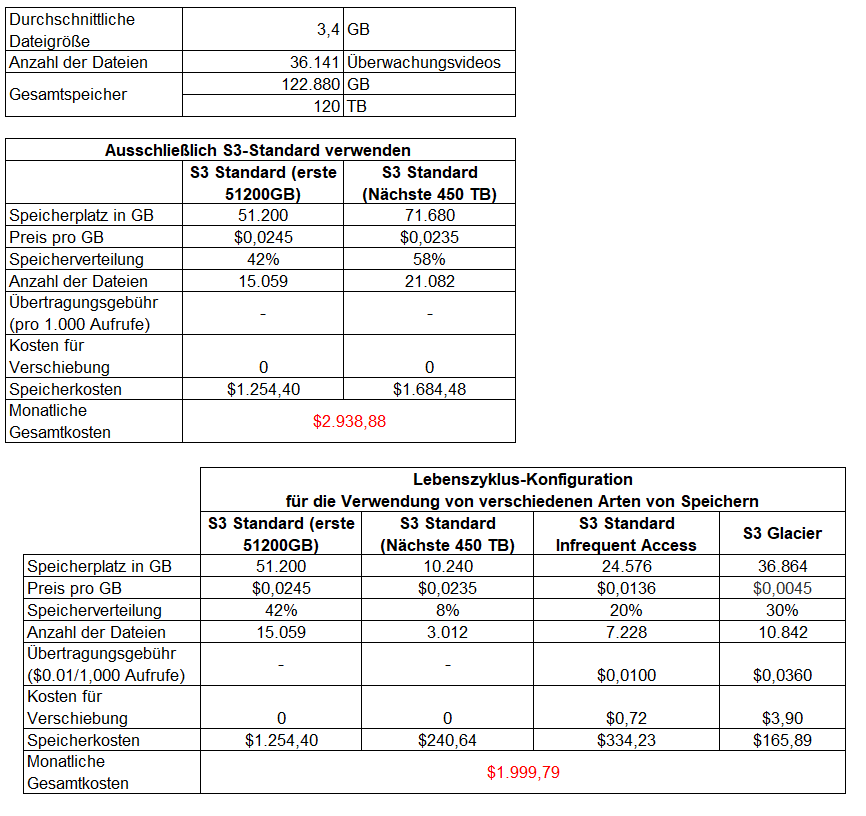
\includegraphics[scale=0.7]{sources/Kostenvergleich_Nutzung_unt_Speicherklassen}
  \caption[Kostenvergleich durch Nutzung von unterschiedlichen Speicherklassen]{}\label{fig:Kostenvergleich_Nutzung_unt_Speicherklassen} 
  Kostenvergleich durch Nutzung von unterschiedlichen Speicherklassen. \\ 
  Quelle: Eigene Darstellung mit Stundensätze der S3-Preise.(Vgl. AWS, 2021, AWS S3 Pricing, o.S.\cite{AMZ09})
\end{figure}
\begin{flushleft}
Anhand der Berechnungen in der \autoref{fig:Kostenvergleich_Nutzung_unt_Speicherklassen} wird sichtbar, dass ein Einsparungspotenzial von rund 1.000 (Eintausend) USD pro Monat besteht.\footnote{Bei der Berechnung wurden die Kosten für das Verschieben von Videos zwischen Speicherklassen berücksichtigt.} Die notwendigen Regeln für die Verschiebung von den Videos erfolgt mit Hilfe einer Lebenszyklus-Konfiguration\footnote{Eine ähnliche Lebenszyklus-Konfiguration, wie die von Unterkapitel \ref{ssec:Lebenszyklus-Konfiguration}} und somit wird ein Teil der Videos in anderen kostengünstigeren Speicherklassen verschoben.
\end{flushleft}
%WICHTIG IST DIE GRÖSSE MEINE DATEIEN UND DIE ANZAHL.
%weil SO WERDEN DIE PREISE FÜR VERSCHIEBUNG BERECHNET.
%(Object size distribution )
\newpage
\subsubsection{Intelligent-Tiering}
Das \textit{Intelligent-Tiering} verschiebt Objekte auf der Grundlage von Zugriffsmustern. Diese Speicherklasse ist ideal für Objekte mit wechselnden oder unbekannten Zugriffsmustern. Wie die Senior Product Managerin für Amazon S3 \textit{Ruhi Dang} erklärt, hätten einige Unternehmen weder die Zeit noch das Geld, um eine Person einzustellen, die ihre Daten sortiert und in die richtige Speicherklasse einordnet\footnote{Vgl. Ruhi Dang, 2019, AWS re:Invent 2019: Guidelines and design patterns for optimizing cost in Amazon S3. Minute: 20:05 \cite{AMZ16}}. Intelligent-Tiering ist eine attraktive Lösung für Unternehmen, die jährlich weniger als 100,000 USD für Speicher ausgeben. \footnote{Vgl. Ruhi Dang, 2019, AWS re:Invent 2019: Guidelines and design patterns for optimizing cost in Amazon S3. Minute: 21:12 \cite{AMZ16}}
%Ach von Jessie Felix gesagt https://www.youtube.com/watch?v=IOT41L_adSw
\\\\
Die \autoref{fig:S3_IntLifeCycle} zeigt, wie Objekte in Abhängigkeit davon, ob auf sie zugegriffen wurde oder nicht, verschieben werden. 
\begin{figure}[h!]
  \centering
  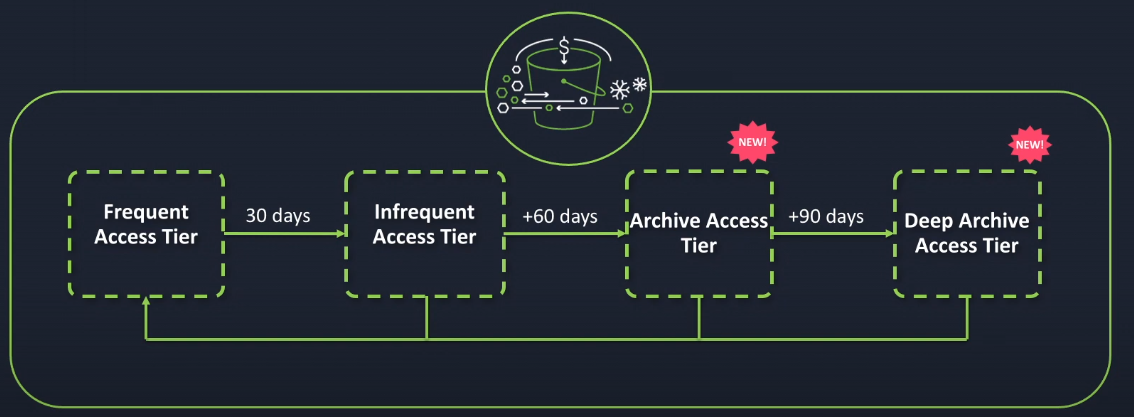
\includegraphics[scale=0.6]{sources/S3_IntLifeCycle}
  \caption[Funktionsweise von Intelligent-Tiering]{}\label{fig:S3_IntLifeCycle} Funktionsweise von Intelligent-Tiering
  %{\cite{SCOUT1}}
\end{figure}\\
Quelle: Eigene Darstellung auf der Grundlage von \\
der Funktionsweise von Intelligent-Tiering.\footnote{Vgl. AWS, 2021, Amazon Simple Storage Service - User Guide. S.715\cite{AMZ18}}
\\\\
Wird ein Objekt zu einem späteren Zeitpunkt aus der Ebene der seltenen Zugriffe aufgerufen, wird dieses automatisch in eine Speicherklasse der häufigen Zugriffe zurückversetzt.
%TALVEZ PARA RELLENAR UN POCO HACER UN CALCULO DE CUANTO SALDRIA SI SE USA Intelligent-Tiering para el caso de los videos
%En comparación con Lebenszyklus-Konfiguration Intelligent-Tiering objetos son regresados al ser llamados/usados.
%Ademas los tiempos de desplazamientos ya están definidos en Intelligent-Tiering.
%Anwenfungsbeispiel?
%Intelligent-Tiering bietet die Möglichkeit, Objekte in fünf verschiedenen Ebenen zu verschieben. 
\subsubsection*{Anwendungsbeispiel Intelligent-Tiering} 
Im Folgenden wird eine Berechnung mit Intelligent-Tiering für das Szenario über die Sicherheitsvideos des Unterkapitels \ref{Anwendungsbeispiel-Leben-Konfig} durchgeführt. In diesem Fall wurden ausschließlich die Ebenen \textit{Frequent-Access, Infrequent-Access} und \textit{Instant-Archive-Access} ausgewählt.\footnote{Da bei der Berechnung des Unterkapitels \ref{Anwendungsbeispiel-Leben-Konfig} eine Speicherklasse für häufigen Zugriff, eine für seltenen Zugriff und eine für Archivierung verwendet wurde, wurden vergleichbare Speicherebenen für die Berechnung mit Intelligent-Tiering ausgewählt.} %Die Ebenen \textit{Archive-Access} und \textit{Deep-Archive-Access} wurden vernachlässigt. %nicht berücksichtigt
\\\\
Die Speicherzuweisung für die 120 TB in den Speicherebenen wurde wie folgt:\\
Frequent-Access-Tier: 50\% \\
Infrequent-Access-Tier: 20\%\\
Instant-Archive-Access: 30\%
\\
\begin{figure}[h!]
  \centering
  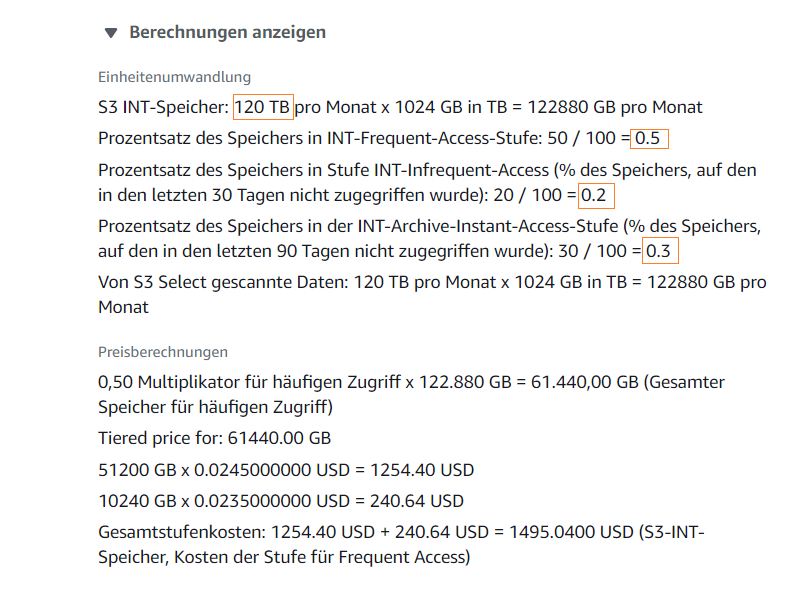
\includegraphics[scale=0.6]{sources/S3_INT_1}
  \caption[Berechnung für die Verwaltung von 120 TB mit AWS Pricing-Calculator für S3 Intelligent-Tiering (1)]{}
  \label{fig:INT_S3_1} Berechnung für die Verwaltung von 120 TB mit AWS Pricing-Calculator für S3 Intelligent-Tiering f(1).\\
  Quelle: eigene Darstellung von AWS Pricing-Calculator \cite{AMZ17-S3}.
  %{\cite{SCOUT1}}
\end{figure}
\newpage
In der \autoref{fig:INT_S3_2} werden die Kosten gezeigt, die durch jede Speicherebene anfallen (Orange markiert). 
\\
Darüber hinaus werden die folgenden Kosten berechnet (Blau markiert): \\
- Überwachung und Automatisierung von 36.141 Objekten.\\
- Leseanfragen (GET-Anfragen) von 18.070 Objekten, welche 50\% der Gesamtzahl der Videos entsprechen, wie in den Anforderungen im Unterkapitel \ref{Anwendungsbeispiel-Leben-Konfig} definiert. \\
- Scannen von Objekten, die allen Videos und 120 TB entsprechen.
\\
\begin{figure}[h!]
  \centering
  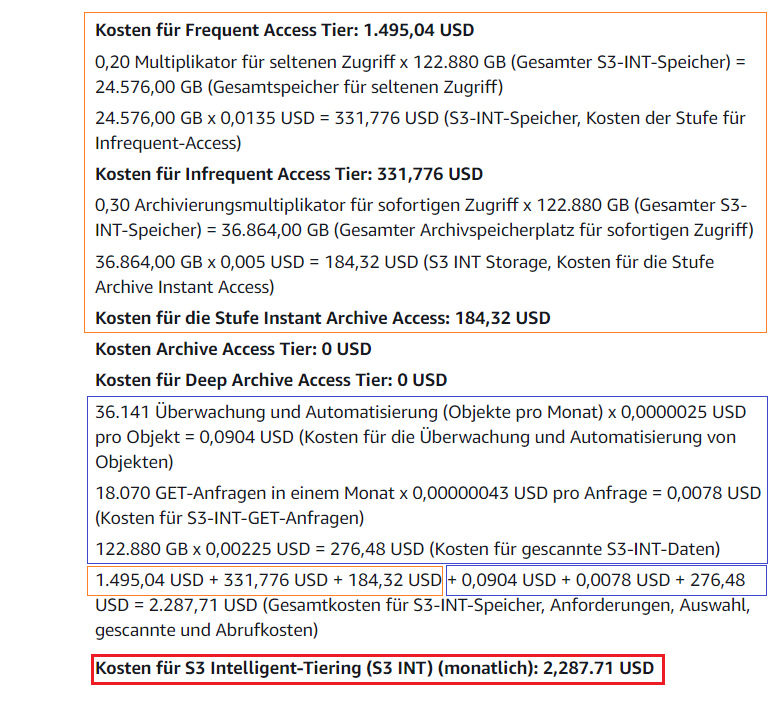
\includegraphics[scale=0.6]{sources/S3_INT_2}
  \caption[Berechnung für die Verwaltung von 120 TB mit AWS Pricing-Calculator für S3 Intelligent-Tiering (2)]{}
  \label{fig:INT_S3_2} Berechnung für die Verwaltung von 120 TB mit\\ AWS Pricing-Calculator für S3 Intelligent-Tiering (2).\\
  Quelle: eigene Darstellung mit AWS Pricing-Calculator \cite{AMZ17-S3}.
\end{figure}
\newpage
\subsubsection*{Vergleich zwischen der Intelligent-Tiering und der Lebenszyklus-Konfiguration}%[Rev]
Bezüglich dieser Thematik muss betont werden, dass bei Intelligent-Tiering die Objekte in Ebenen von seltenen Zugriff automatisch auf eine Ebene für häufigen Zugriff zurückgegeben werden. Siehe \autoref{fig:S3_IntLifeCycle}.
\\\\
Ein weiterer Unterschied liegt darin, dass bei einer Lebenszyklus-Konfiguration die Tage der Verschiebung zwischen den Speicherklassen und die Speicherklassen leicht verändert werden können. Diese ist bei Intelligent-Tiering standardmäßig vorab bereits festgelegt. %Die Möglichkeit die Zeitabstand für die Verschiebung zwischen Ebenen bei Intelligent-Tiering wurde in der AWS-Dokumentation nicht gefunden. 
Darüber hinaus besteht die Möglichkeit, Objekte aus Intelligent-Tiering in andere Speicherklassen zu verschieben, %(mit Einschränkungen),
indem man eine Lebenszyklus-Konfiguration verwendet.\footnote{Vgl. AWS, 2021, Amazon Simple Storage Service - User Guide. S.724.\cite{AMZ18}} %t.ly/1CgV
Dadurch wäre es möglich Objekte für einen längeren Zeitraum in einer bestimmten Speicherklasse aufzubewahren und Richlinien von Intelligent-Tiering zu überspringen.
%COMMENTS
\begin{comment}
\subsubsection{Automatisierung mit Lambda Funktionen}
Grund: einmal programmiert, funktioniert es für immer.
\\(To-Do:) Möglichkeiten untersuchen, bewerten und die passende Auswählen.

%Limitierung 
%Quotas setzen? erweitern oder reduzieren / benachrichtigen aber auch eine Aktion durchführen 
%Lambda

AWS Lambda is a compute service. You can use it to run code without provisioning or managing servers. Lambda runs your code on a high-availability compute infrastructure. It operates and maintains all of the compute resources, including server and operating system maintenance, capacity provisioning and automatic scaling, code monitoring, and logging. With Lambda, you can run code for almost any type of application or backend service. 

Some benefits of using Lambda include the following:

You can run code without provisioning or maintaining servers.
It initiates functions for you in response to events.
It scales automatically.
It provides built-in code monitoring and logging via Amazon CloudWatch.
\end{comment}

%Data Pipeline

%Economic Performance?
%QUEUES

%NEVER forget your availability requirements, trying to optimize, first availability THEN cost...
%Do not use your DB for saving BLOB

%\subsection{VERKAUFE DEINE Ungenutzte Kapazität in RI Marketplace}

%Kombination
%https://spot.io/blog/effective-utilization-of-aws-savings-plans-and-ec2-spot-instances/#a1
%https://www.youtube.com/watch?v=X_7pnzPlESs

 